\section{Glaziale Geomorphologie}
\subsection{Geomorphologie}
\begin{myexercise}
Notieren Sie sich beim Anschauen des Films, welche Formen genannte werden und beantworten Sie folgende Fragen:
\begin{itemize}
\item Wo entsteht ein Gletscher typischerweise? Was ist ein Kar?
\item Wie entsteht ein Gletscher? Welche Zwischenstadien werden genannt von Schnee bis Eis?
\item Wie bewegt sich der Gletscher talwärts? Um wie viel können sich Gletscher bewegen?
\item Was ist eine Glaziale Serie? Welche Landschaftsformen gehören dazu?
\item Beschreiben Sie folgende Landschaftsformen: Drumlin, Seitenmoräne, Endmoräne, Grundmoräne, Zungenbeckensee, Schotterfeld
\end{itemize}
\end{myexercise}
\notiz{8}

\begin{myexercise}
Annotieren Sie folgene Modelle anhand der Bilder und Begriffe, die Ihnen verteilt werden. 
\begin{figure}[H]
\centering
\includegraphics[width=\linewidth]{"Private/Images/Geomorphologie/Modell hep AI leer"}
\caption{Abgeändertes Modell nach \cite{hep}}
\label{fig:modell-hep-ai-leer}
\end{figure}

\begin{figure}[H]
\centering
\includegraphics[width=\linewidth]{"Private/Images/Geomorphologie/Modell Westermann leer"}
\caption{Abgeändertes Modell nach \cite{westermann}}
\label{fig:modell-westermann-ai-leer}
\end{figure}
\end{myexercise}

\subsection{Massenbilanz eines Gletschers}

Die \textbf{Massenbilanz} eines Gletschers, auch \textbf{Gletscherhaushalt} genannt, beschreibt die Differenz zwischen der \textbf{Akkumulation} (Massenaufnahme) und der \textbf{Ablation} (Massenverlust) innerhalb eines bestimmten Zeitraums. Sie ist ein entscheidender Faktor für das Wachstum oder den Rückzug eines Gletschers und wird von verschiedenen klimatischen und physikalischen Prozessen beeinflusst.

\subsubsection{Akkumulationsgebiet (Nährgebiet) und Ablationsgebiet (Zehrgebiet)}

Ein Gletscher kann in zwei Hauptzonen unterteilt werden: das \textbf{Akkumulationsgebiet} (oder \textbf{Nährgebiet}) und das \textbf{Ablationsgebiet} (oder \textbf{Zehrgebiet}). 

Im Akkumulationsgebiet sammelt sich neue Masse durch Schneefall an, der im Laufe der Zeit durch Druck zu Firn, Firneis und schliesslich zu Gletschereis verdichtet wird. Dieses Gebiet liegt typischerweise in den höheren Lagen eines Gebirgsgletschers, wo die Temperaturen niedrig genug sind, dass der Schnee ganzjährig liegenbleibt und sich fortlaufend kompaktiert (s. \cref{fig:akkumulation}). Akkumulation kann nicht nur durch Schneefall erfolgen, sondern auch durch gefrierenden Regen, Eisansammlung durch Lawinen oder durch Windverfrachtung von Schnee. 

\begin{figure}[H]
\centering
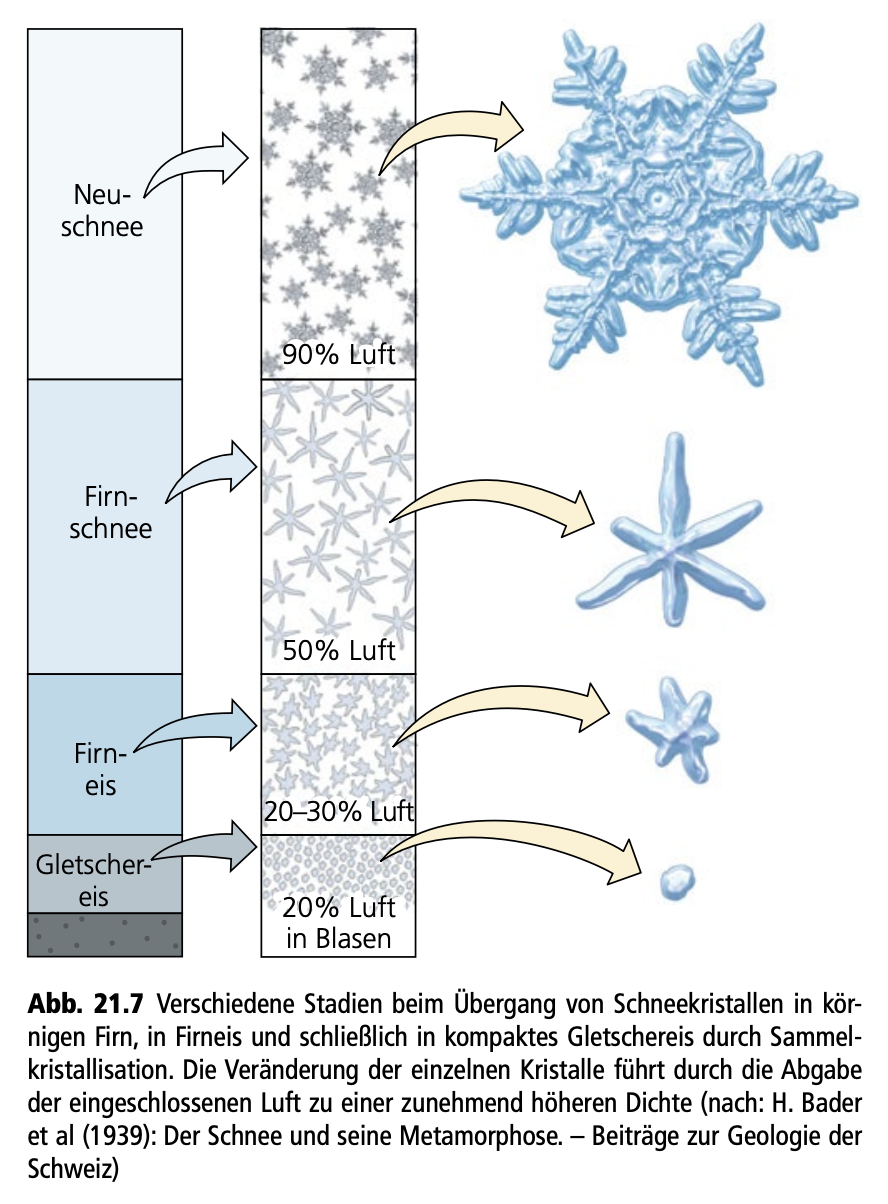
\includegraphics[width=0.5\linewidth]{Private/Images/Geomorphologie/Akkumulation}
\caption{Metamorphose von Schnee zu Eis \cite{allgemeineGeologie}}
\label{fig:akkumulation}
\end{figure}

Das Ablationsgebiet hingegen ist der Bereich des Gletschers, in dem mehr Masse verloren geht als hinzukommt. Ablation erfolgt hauptsächlich durch Schmelze, aber auch durch Sublimation, also den direkten Übergang von Eis in Wasserdampf. Dieser Bereich befindet sich in tieferen Lagen, wo die Temperaturen im Sommer oft über dem Gefrierpunkt liegen und somit zur Abschmelzung des Eises beitragen.

\begin{figure}[H]
\centering
\includegraphics[width=0.7\linewidth]{"Private/Images/Geomorphologie/Akkumulation und Ablation"}
\caption{Akkumulations- und Ablationsgebiete, nach \cite{allgemeineGeologie}}
\label{fig:akkumulation-und-ablation}
\end{figure}


\subsubsection{Firnlinie und Gleichgewichtslinie}

Zwischen dem Akkumulations- und dem Ablationsgebiet liegt die \textbf{Firnlinie}, die den Übergang zwischen dem Bereich mit mehrjährigem Schnee und dem Bereich mit reinem Gletschereis markiert. Diese Linie ist manchmal, aber nicht immer, von blossem Auge erkennbar, wie etwas in \cref{fig:gleichgewichtslinie-3}.

\begin{figure}[H]
\centering
\includegraphics[width=0.7\linewidth]{"Private/Images/Geomorphologie/Gleichgewichtslinie 3"}
\caption{Gleichgewichtslinie und Firnlinie eines Gletschers nach \cite{gletscherOnline}}
\label{fig:gleichgewichtslinie-3}
\end{figure}.

Die \textbf{Gleichgewichtslinie} markiert den Punkt, an dem die jährliche Massenzunahme durch Akkumulation genau der jährlichen Massenabnahme durch Ablation entspricht. Die Position dieser Linie variiert von Jahr zu Jahr und ist ein wichtiger Indikator für klimatische Veränderungen.

\subsubsection{Jährliche Veränderung der Position und Klimaeinfluss}

Die Position der Gleichgewichtslinie ist nicht konstant, sondern verändert sich in Abhängigkeit von klimatischen Bedingungen wie Temperatur und Niederschlagsmenge. Eine klimatische Erwärmung führt dazu, dass die Gleichgewichtslinie auf höhere Höhenlagen ansteigt, da das Ablationsgebiet sich ausdehnt. Umgekehrt kann eine Abkühlung des Klimas dazu führen, dass die Gleichgewichtslinie absinkt und sich das Akkumulationsgebiet vergrössert. Dadurch bedingt sinkt auch das Ablationsgebiet nach unten und der Gletscher wird grösser, bzw. länger. Diese jährlichen Schwankungen sind direkte Folgen von klimatischen Bedingungen und beeinflussen die langfristige Entwicklung des Gletschers.

\subsubsection{Temperaturen, Schneefall und Gletscherbewegung}

Die Massenbilanz eines Gletschers wird massgeblich von Temperaturen und Schneefall bestimmt. Hohe Temperaturen verstärken die Schmelze und Sublimation, während niedrige Temperaturen die Akkumulation fördern. Die Menge und Verteilung des Schneefalls beeinflusst, wie viel Masse im Akkumulationsgebiet gespeichert wird. Neben der Massenbilanz spielt auch die Gletscherbewegung eine wichtige Rolle. Durch die Schwerkraft fliesst das Eis langsam talwärts, wobei interne Deformationen im Eiskörper (plastisches Fliessen) und das Gleiten auf dem flüssigen Untergrund (Sohlgleitung) die Hauptmechanismen sind (s. \cref{fig:gleiten-und-fliessen-gletscher-crop}).


\begin{figure}[H]
\centering
\includegraphics[width=0.9\linewidth]{"Private/Images/Geomorphologie/Gleiten und Fliessen Gletscher crop"}
\caption{Bewegungsprozesse von Gletschern nach \cite{allgemeineGeologie}}
\label{fig:gleiten-und-fliessen-gletscher-crop}
\end{figure}

\begin{figure}[H]
\centering
\includegraphics[width=0.9\linewidth]{"Private/Images/Geomorphologie/Gleiten und Fliessen Gletscher 2"}
\caption{Plastisches Fliessen: Detailansicht}
\label{fig:gleiten-und-fliessen-gletscher-2}
\end{figure}


Die Sohlgleitung kommt dadurch zustande, dass Eis bei gleichbleibender Temperatur unter Druck flüssig werden kann (s. \cref{fig:tripelpunkt}).

\begin{figure}[H]
\centering
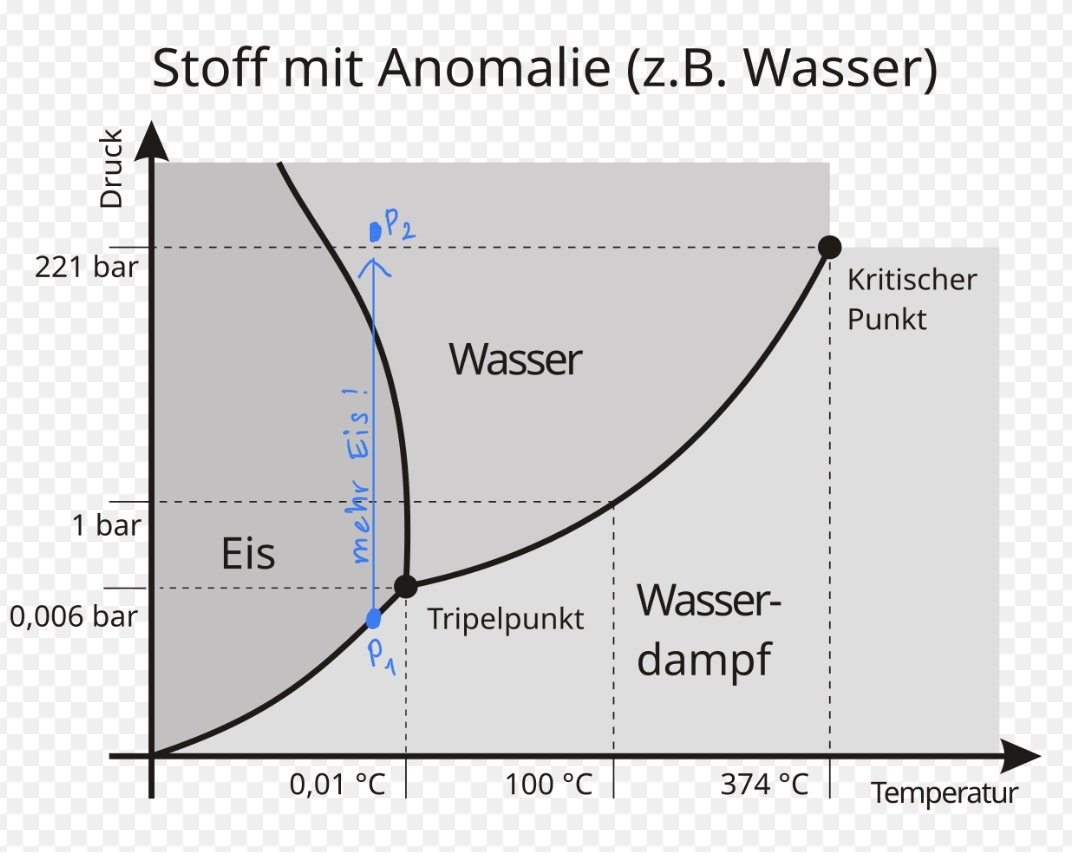
\includegraphics[width=0.7\linewidth]{Private/Images/Geomorphologie/Tripelpunkt}
\caption{Tripelpunkt: $P_1$ = Eis auf der Gletscheroberfläche, $P_2$ = Eis am Boden des Gletschers wird zu Wasser}
\label{fig:tripelpunkt}
\end{figure}


\subsection{Reaktionszeit eines Gletschers}

Die Reaktionszeit eines Gletschers beschreibt, wie schnell er auf Veränderungen in der Massenbilanz reagiert. Kleine Gletscher mit steilen Hängen passen sich relativ schnell an klimatische Veränderungen an, während grosse Gletscher mit flachen Neigungen eine längere Reaktionszeit haben. Diese Verzögerung kann dazu führen, dass Gletscher noch Jahrzehnte nach einer Klimaveränderung weiter wachsen oder schrumpfen, selbst wenn sich das Klima bereits verändert hat.

\begin{myexercise}
Lösen Sie folgendes Quiz: \qrcode{https://wendl.ch/quiz-gletscher}
\end{myexercise}

\begin{myexercise}[9 Testfragen]
\begin{enumerate}
\item Erklären Sie in ganzen Sätzen, was ein Gletscher ist und wie er sich ernährt.

\item Beschreiben Sie in ganzen Sätzen, wie ein Gletscherzungensee entsteht.
\item Beschreiben Sie in ganzen Sätzen, wie sich ein Gletscher bewegt.
\item Erläutern Sie den Unterschied zwischen einem Rundhöcker und einem Drumlin.
\item Erstellen Sie eine Legende zur untenstehenden Abbildung. Wählen Sie dazu selber zehn Begriffe aus und schreiben Sie die Zahl an die richtige Stelle in der Abbildung.
\item Nennen Sie zwei Gletschergefahren und zwei Gletschernutzungen.
\item Erläutern Sie den Unterschied zwischen einem Hängetal und einem Trogtal.
\item Erklären Sie den Begriff ``Ablation''.
\item Begründen Sie in ganzen Sätzen, weshalb die Eiszeit ein Segen für die heute hier lebenden Menschen darstellt.
\end{enumerate}
\begin{figure}[H]
\centering
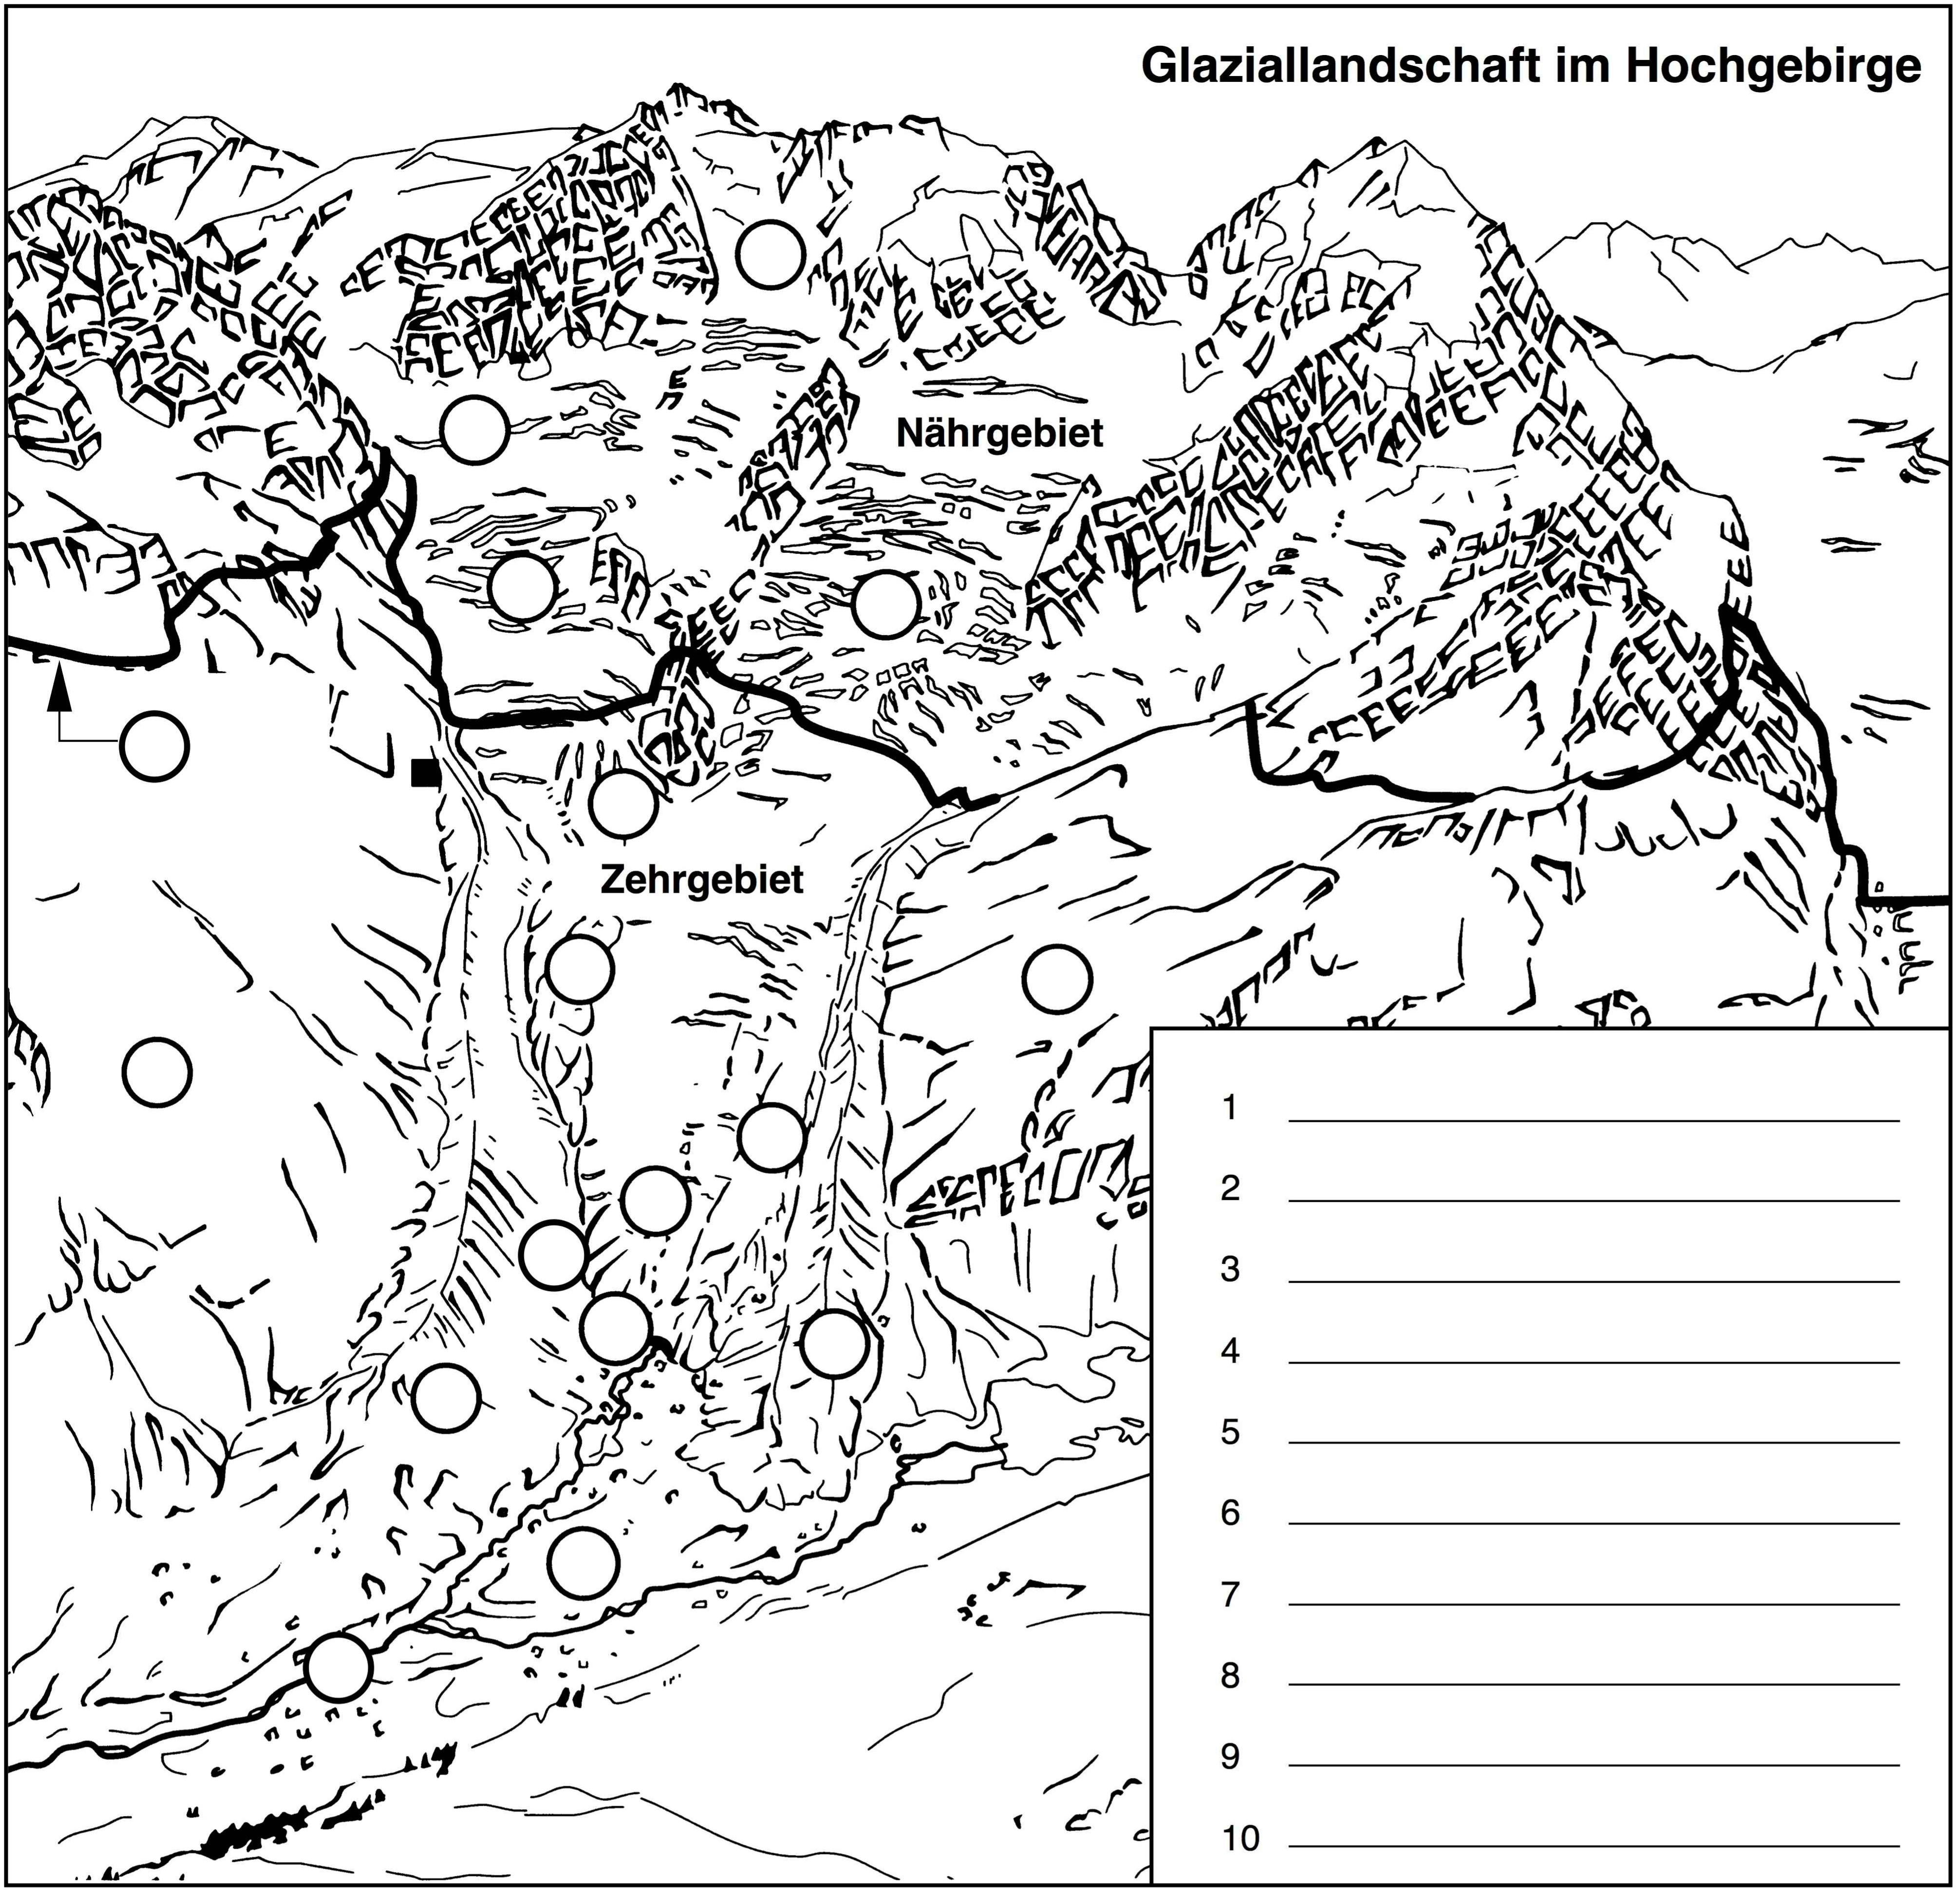
\includegraphics[width=0.7\linewidth]{Private/Images/Geomorphologie/Leer-Bild}
\end{figure}


\end{myexercise}
\begin{mychallenge}[Lehrbuchtext zu glazialen Formen]
\foreach \pagenum in {1,...,6} {
\begin{figure}[H]
\centering
\includegraphics[width=0.9\linewidth, page=\pagenum]{"Geografie/Diercke Geografie Geomorphologie"}
\caption{Glaziale Geomorphologie \cite{westermann}}
\end{figure}
}

\end{mychallenge}



\newpage

\section*{Lernziele DL 1}

\begin{todolist}
\item Ich kann zwischen Verwitterungs- und Erosionsprozessen unterscheiden
\item Ich kann zwischen physikalischer, chemischer, und chemisch-physikalischer Erosion unterscheiden
\item Ich kann physikalische (Temperatur, Frost, Salz, Druck, Bio-Physikalisch) und chemische (Lösung, Oxidation, Hydratation, Biologisch-Chemische) Verwitterungsprozesse zu geomorphologischen Formen zuordnen.
\end{todolist}

\section*{Lernziele DL 2}
\begin{todolist}
\item Ich kann die geologischen Faktoren, die zum Entstehen von Kerbtälern (auch V-Täler genannt), Schluchten sowie Canyons führen, auflisten und erklären.
\item Ich kann die baulichen Herausforderungen, welche in Kerbtälern entstehen anhand folgender Begriffe erklären:  Hangrutschung, Fundament, Verstärkung, Brücken.
\item Ich kann das Entstehen von Mäandern erklären, indem ich Begriffe verwende: Prallhang, Gleithang, Tiefenerosion, Seitenerosion
\item Ich kann die Entstehung von Flussdeltas anhand folgender fluvialer Prozesse erklären: Fliessgeschwindigkeit, Erosion und Ablagerung.
\end{todolist}
\section*{Lernziele DL 3}

\begin{todolist}
\item Ich kann die Entstehung von Gletschern beschreiben, indem ich folgende Begriffe verwende und einem Bild zuordne: \textit{Kar, Schnee, Firn, Firneis, Eis, Volumen, Verdichtung}
\item Ich kann folgende geläufige geomorphologische Formen auf Fotos sowie Modellen einordnen und deren Entstehung erklären:
\begin{todolist}
\item \textbf{Ablagerungs-Formen}: Seitenmoräne, Grundmoräne, Endmoräne, Mittelmoräne, Drumlin, Erratiker (auch Findling, erratischer Block)
\item \textbf{Tal-Typen}: Hängetal, Trogtal (auch U-Tal genannt), Kar, Schliffgrenze
\item \textbf{Glaziale Serie}: Grundmoräne, Zungenbecken, Zungenbeckensee, Schotterfeld, Toteissee
\item \textbf{Gletscher-Formen}: Längs-, Quer-, Seiten- und Radialspalten, Gletschertisch, Gletscherbach, Gletschertor, Gletscherzunge, Zungenbecken(-see), Bergschrund
\item \textbf{Weitere Formen}: Rundhöcker, Schrammen
\end{todolist}
\item Ich kenne die Begriffe Ablation und Akkumulation und kann Einfluss-Faktoren für beide Prozesse benennen und erklären.
\item Ich kann die Veränderung der Massenbilanz eines Gletschers aufgrund des Klimas beschreiben, indem ich die Begriffe \textit{Nährgebiet}, \textit{Zehrgebiet}, \textit{Gleichgewichtslinie} und \textit{Firnlinie}, \textit{Schneefall}, \textit{Sublimation} und \textit{Resublimation} verwende.
\end{todolist}

